%!TEX program = xelatex 

% Documentation for pkuthss.
%
% Copyright (c) 2008-2009 solvethis
% Copyright (c) 2010-2016,2018-2019 Casper Ti. Vector
%
% This work may be distributed and/or modified under the conditions of the
% LaTeX Project Public License, either version 1.3 of this license or (at
% your option) any later version.
% The latest version of this license is in
%   https://www.latex-project.org/lppl.txt
% and version 1.3 or later is part of all distributions of LaTeX version
% 2005/12/01 or later.
%
% This work has the LPPL maintenance status `maintained'.
% The current maintainer of this work is Casper Ti. Vector.
%
% This work consists of the following files:
%   pkuthss.tex
%   chap/pkuthss-copy.tex
%   chap/pkuthss-abs.tex
%   chap/pkuthss-intro.tex
%   chap/pkuthss-chap1.tex
%   chap/pkuthss-chap2.tex
%   chap/pkuthss-chap3.tex
%   chap/pkuthss-concl.tex
%   chap/pkuthss-encl1.tex
%   chap/pkuthss-ack.tex

\documentclass[UTF8, AutoFakeBold]{pkuthss}
\usepackage[
	backend = biber, style = caspervector, utf8, 
	%sorting = none,
	giveninits = true, sortgiveninits = true]{biblatex}
\usepackage{iftex, fancyvrb, hologo}
\usepackage{booktabs}
\usepackage{multirow}
\usepackage{pdfpages}

\hypersetup{colorlinks = true, allcolors = black}
\ctexset{linestretch = 0\ccwd}
\setlength{\hfuzz}{3pt}
\setlength{\bibitemsep}{3bp}
\renewcommand*{\bibfont}{\zihao{5}\linespread{1.27}\selectfont}
\newcommand*{\cupercite}[1]{\supercite{#1}\mbox{}}
\newcommand{\myemph}[1]{\emph{\textcolor{red}{#1}}}
\newcommand{\unemph}[1]{\textup{\textcolor{black}{#1}}}
\newcommand{\RNum}[1]{\rm\uppercase\expandafter{\romannumeral #1}}
\renewcommand{\cftchapfont}{\songti\zihao{-4}}%目录
\renewcommand{\cftsecfont}{\songti\zihao{-4}} %设置section条目的字体
\renewcommand{\cftsubsecfont}{\songti\zihao{-4}} %设置subsection条目的字体
\renewcommand{\listfigurename}{图目录}
\renewcommand{\listtablename}{表目录}
\RecustomVerbatimEnvironment{Verbatim}{Verbatim}%
	{frame = single, tabsize = 4, formatcom = {\ifXeTeX\xeCJKVerbAddon\fi}}
\RecustomVerbatimCommand{\VerbatimInput}{VerbatimInput}{
	fontsize = {\small}, baselinestretch = 1,
	tabsize = 4, formatcom = {\ifXeTeX\xeCJKVerbAddon\fi}
}

\makeatletter
\newcommand\engcontentsname{CONTENTS}
\newcommand\tableofengcontents{%
    \if@twocolumn
      \@restonecoltrue\onecolumn
    \else
      \@restonecolfalse
    \fi
    \chapter*{\engcontentsname
        \@mkboth{
           \MakeUppercase\engcontentsname}{\MakeUppercase\engcontentsname}}
    \@starttoc{toe}
    \if@restonecol\twocolumn\fi
    }
\newcommand\addengcontents[2]{
    \addcontentsline{toe}{#1}{\protect\numberline{\csname the#1\endcsname}#2}}
\makeatother
\newcommand\echapter[1]{\addengcontents{chapter}{#1}}
\newcommand\esection[1]{\addengcontents{section}{#1}}
\newcommand\esubsection[1]{\addengcontents{subsection}{#1}}
\newcommand\esubsubsection[1]{\addengcontents{subsubsection}{#1}}

\newcommand*{\docversion}{v1.8.2}
\pkuthssinfo{
	fenleihao={O572},
	miji={公开},
	danweidaima={10422},
	xuehao={200000000},
	cthesisname = {硕\hspace{0.5em}士\hspace{0.5em}学\hspace{0.5em}位\hspace{0.5em}论\hspace{0.5em}文}, ethesisname = {Thesis\hspace{0.5em}for\hspace{0.5em}Master\hspace{0.5em}Degree},
	ctitle = {喵喵喵喵喵喵},
	etitle = {%
	            miaomiaomiaomiaomiaomiao\texorpdfstring{\\}{: }%
	},
	cauthor = {Arisukawa},
	eauthor = {Arisukawa},
	studentid = {200000000},
	date = {2021年4月5日},
	school = {前沿交叉科学青岛研究院},
	cmajor = {物理学}, emajor = {Physics Major},
	direction = {粒子物理与原子核物理},
	cmentor = {ZYC教授}, ementor = {Prof. ZYC},
	comentor = {},
	ckeywords = {喵1;喵2;喵3;喵4;喵5},
	ekeywords = {miao1; miao2; miao3; miao4; miao5},
}

\addbibresource{pkuthss.bib}

\begin{document}
	\frontmatter
	\pagestyle{empty}
    \maketitle
	\cleardoublepage

	\cleardoublepage
	\pagenumbering{gobble}
	\pagestyle{plain} 
	\thispagestyle{empty}

\begin{spacing}{2}
{\zihao{4}

\vspace*{1.cm}

\phantomsection
\addcontentsline{toc}{chapter}{原创性声明和关于论文使用授权的声明}
\addcontentsline{toe}{chapter}{STATEMENT}

\centerline{\heiti 原~ 创~ 性~ 声~ 明}

本人郑重声明:所呈交的学位论文,是本人在导师的指导下,独立进
行研究所取得的成果。除文中已经注明引用的内容外,本论文不包含任何
其他个人或集体已经发表或撰写过的科研成果。对本文的研究作出重要贡
献的个人和集体,均已在文中以明确方式标明。本声明的法律责任由本人
承担。

论文作者签名:\underline{\hspace{5\ccwd}}
~~~
日 期:\underline{\hspace{5\ccwd}}





\vskip\baselineskip
\vskip\baselineskip











\centerline{\heiti 关于学位论文使用授权的声明}



本人同意学校保留或向国家有关部门或机构送交论文的印刷件和电子
版,允许论文被查阅和借阅;本人授权山东大学可以将本学位论文的全部
或部分内容编入有关数据库进行检索,可以采用影印、缩印或其他复制手
段保存论文和汇编本学位论文。

(保密论文在解密后应遵守此规定)

\noindent
~
论文作者签名:\underline{\hspace{5\ccwd}}
~~
导师签名:\underline{\hspace{5\ccwd}}
~~
日~~期:\underline{\hspace{5\ccwd}}



}
\end{spacing}


	\tableofcontents
    \tableofengcontents
    \listoffigures
    \listoftables
    \cleardoublepage

	\cleardoublepage
    \pagestyle{plain} 
    \setcounter{page}{0}
    \pagenumbering{Roman}
    % Documentation for pkuthss.
%
% Copyright (c) 2008-2009 solvethis
% Copyright (c) 2010-2014 Casper Ti. Vector
%
% This work may be distributed and/or modified under the conditions of the
% LaTeX Project Public License, either version 1.3 of this license or (at
% your option) any later version.
% The latest version of this license is in
%   https://www.latex-project.org/lppl.txt
% and version 1.3 or later is part of all distributions of LaTeX version
% 2005/12/01 or later.
%
% This work has the LPPL maintenance status `maintained'.
% The current maintainer of this work is Casper Ti. Vector.
%
% This work consists of the following files:
%   pkuthss.tex
%   chap/pkuthss-copy.tex
%   chap/pkuthss-abs.tex
%   chap/pkuthss-intro.tex
%   chap/pkuthss-chap1.tex
%   chap/pkuthss-chap2.tex
%   chap/pkuthss-chap3.tex
%   chap/pkuthss-concl.tex
%   chap/pkuthss-encl1.tex
%   chap/pkuthss-ack.tex

\begin{cabstract}
\addcontentsline{toe}{chapter}{ABSTRACT(CHINESE)}
\addcontentsline{toc}{chapter}{摘要}

Hi这里写中文的摘要内容。

\end{cabstract}

\begin{eabstract}
\addcontentsline{toe}{chapter}{ABSTRACT(ENGLISH)}
\addcontentsline{toc}{chapter}{摘要(英文)}

Hi plz put your english abstract here.

\end{eabstract}

% vim:ts=4:sw=4

    \specialchap{符号说明}
\addcontentsline{toe}{chapter}{ABBREVIATION}

\hspace*{1.5cm}	
\begin{tabularx}{0.6\textwidth}{l X l}
			缩写1  &    &听君一席话\\
			缩写2  &    &如听一席话\\
\end{tabularx}


	\mainmatter
	% Documentation for pkuthss.
%
% Copyright (c) 2008-2009 solvethis
% Copyright (c) 2010-2019 Casper Ti. Vector
%
% This work may be distributed and/or modified under the conditions of the
% LaTeX Project Public License, either version 1.3 of this license or (at
% your option) any later version.
% The latest version of this license is in
%   https://www.latex-project.org/lppl.txt
% and version 1.3 or later is part of all distributions of LaTeX version
% 2005/12/01 or later.
%
% This work has the LPPL maintenance status `maintained'.
% The current maintainer of this work is Casper Ti. Vector.
%
% This work consists of the following files:
%   pkuthss.tex
%   chap/pkuthss-copy.tex
%   chap/pkuthss-abs.tex
%   chap/pkuthss-intro.tex
%   chap/pkuthss-chap1.tex
%   chap/pkuthss-chap2.tex
%   chap/pkuthss-chap3.tex
%   chap/pkuthss-concl.tex
%   chap/pkuthss-encl1.tex
%   chap/pkuthss-ack.tex

\chapter{前言}	
\echapter{Introduction}
\section{夸克,胶子和强子}
\esection{Quarks, gluons and hadrons}

以下内容为范例:

夸克和胶子合称部分子,是自然界物质的基础组成部分。夸克之间存在强相互作用力,而色场中的胶子又能联系夸克组成强子,这个过程中的强相互作用能够统一地被量子色动力学(Quantum Chromodynamics, QCD)\parencite{Han:1965pf}所描述。量子色动力学属于非阿贝尔群规范理论\parencite{Gross1973UltravioletBO},其中有两个重要特征:

\begin{itemize}
	\item \textbf{色禁闭\parencite{GellMann:1964nj,Zweig:1964jf}}:喵喵喵
	\item \textbf{渐近自由}:喵喵喵
\end{itemize}

\section{夸克胶子等离子体(QGP)}
\esection{Quark-gluon Plasma}

\begin{figure}[htb]
	\centering
	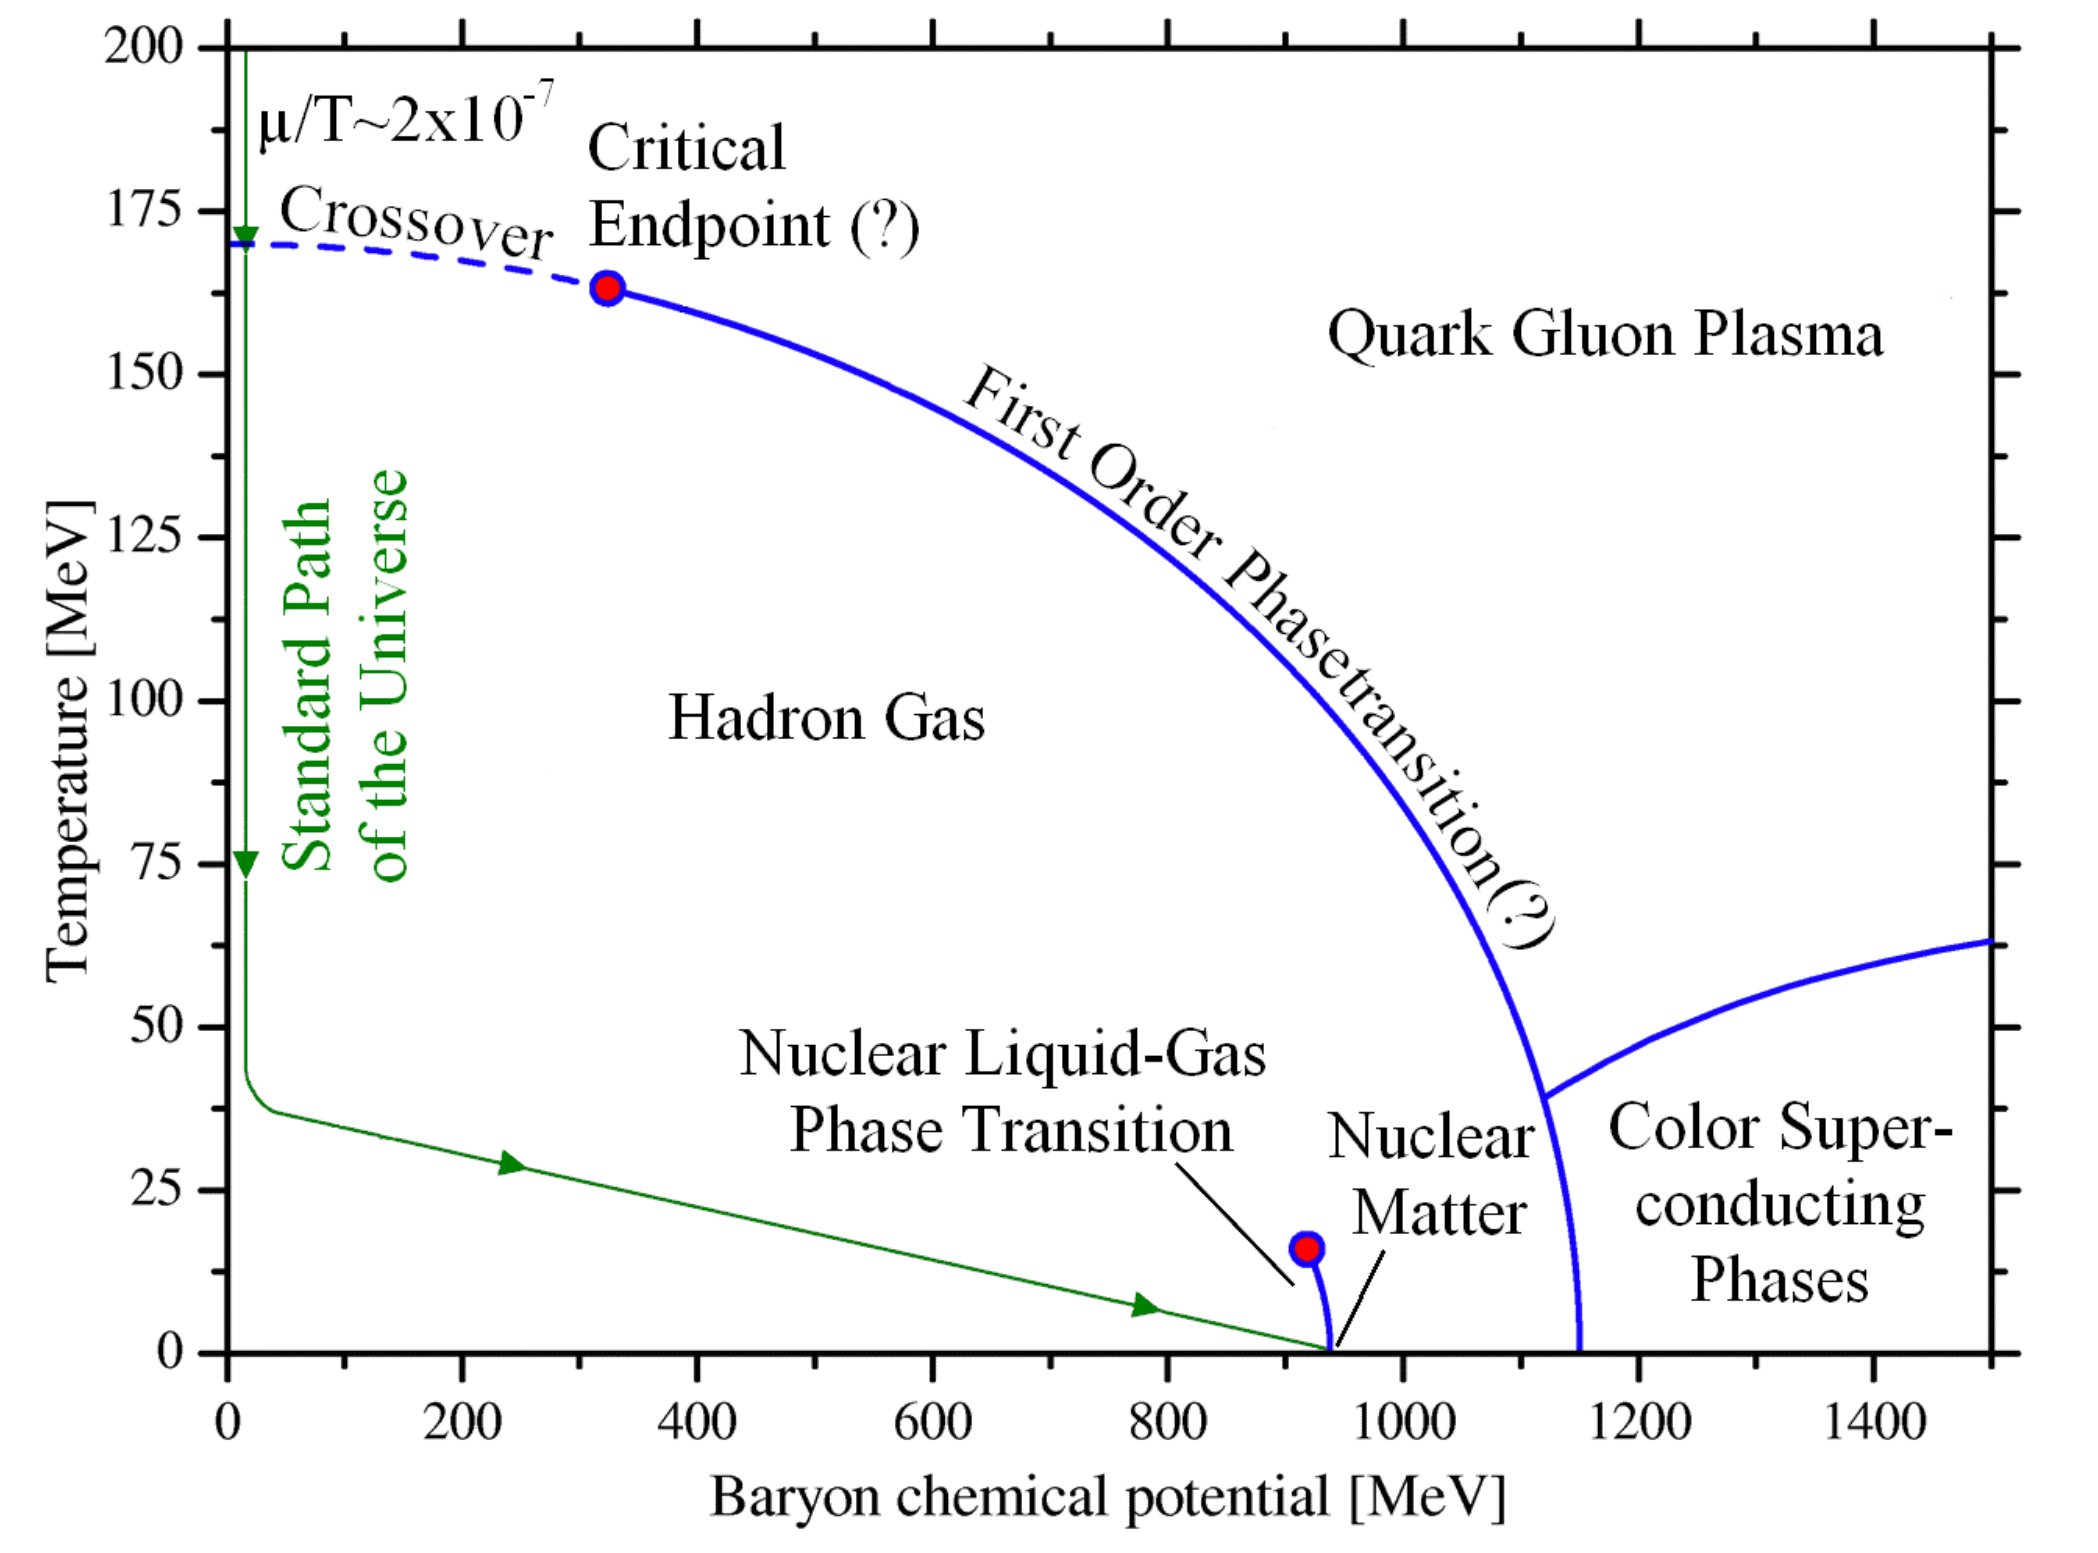
\includegraphics[width=0.7\linewidth]{../figures/1-thesis.png}
	\caption{量子色动力学核物质相变图。~\parencite{Boeckel:2011yj}}
	\label{fig:1-thesis}
\end{figure}

格点量子色动力学对核物质相变做了相关计算并预言了夸克胶子等离子体 ~\parencite{Shuryak:1978ij, Bohr:1977gj, Zajc:2007ey}的存在,QCD相图如图~\ref{fig:1-thesis}
所示,其中也包括许多理论计算推测。相图横轴是与净重子数成正比的净重子化学势,纵轴是温度。夸克胶子等离子体存在于高温(> 150 - 170 MeV)或是高净重子数密度条件下,所以产生QGP的方式既可以是提高核物质的温度,也可以是压缩其体积使净重子数密度提高,或者是两者同时进行。

\section{高能重离子碰撞}
\esection{High Energy Heavy-ion Collisions}

\section{集体流}
\esection{Collective Flow}

\subsection{各种流的现象体现}
\esubsection{Phenomena of Collective Flow}

\subsubsection{径向流(radial flow)}
\esubsubsection{Radial Flow}

\subsection{相对论流体力学模型}
\esubsection{Hydrodynamics Model}
QGP膨胀相关的动力学描述和集体流行为,可以通过量子色动力学的拉格朗日密度描述:

\begin{equation}
\mathit{L}=\overline{\Psi }_{i}(i\gamma_{\mu }\mathit{D}_{ij}^{\mu }-m\delta_{ij})\Psi_{j}-\frac{1}{4} \mathit{F}_{\mu \nu \alpha } \mathit{F}^{ \mu \nu \alpha}
\end{equation}

其中$\Psi_{i}$指夸克场($i$对应不同的色荷状态),$\mathit{D}^{\mu}$是协变导数,$m$是夸克质量,$ \mathit{F}^{ \mu \nu \alpha}$是胶子对应的场强张量,其中$\alpha$对应胶子的色荷状态。

\section{小系统中的集体流行为}
\esection{Collectivity in Small System}

\section{文献综述和论文结构}
\esection{Thesis Structure}


% vim:ts=4:sw=4

	% Documentation for pkuthss.
%
% Copyright (c) 2008-2009 solvethis
% Copyright (c) 2010-2019 Casper Ti. Vector
%
% This work may be distributed and/or modified under the conditions of the
% LaTeX Project Public License, either version 1.3 of this license or (at
% your option) any later version.
% The latest version of this license is in
%   https://www.latex-project.org/lppl.txt
% and version 1.3 or later is part of all distributions of LaTeX version
% 2005/12/01 or later.
%
% This work has the LPPL maintenance status `maintained'.
% The current maintainer of this work is Casper Ti. Vector.
%
% This work consists of the following files:
%   pkuthss.tex
%   chap/pkuthss-copy.tex
%   chap/pkuthss-abs.tex
%   chap/pkuthss-intro.tex
%   chap/pkuthss-chap1.tex
%   chap/pkuthss-chap2.tex
%   chap/pkuthss-chap3.tex
%   chap/pkuthss-concl.tex
%   chap/pkuthss-encl1.tex
%   chap/pkuthss-ack.tex

\chapter{系统误差}
\echapter{Systematic Uncertainty}

\section{“脊”上限中的系统误差}
\esection{Systematic Uncertainties in Ridge Yield Limit}

\begin{table}[htb!]
\renewcommand{\arraystretch}{1.5}
\small
\centering
\begin{tabular}{cccc}
& \multicolumn{3}{l}{\begin{tabular}[c]{@{}c@{}}Systematic Uncertainty Sources \\ in DIS Ridge Yield Limit \\ ( 1.5 < $\Delta\eta$ < 2.0 ) \end{tabular}} \\ \hline
Multiplicity & Charge($\%$) & $Z_{vtx}$($\%$) & Total($\%$)  \\
2  $\leq N_{trk}^{obs}<$ 4 & 0.3 & 0.3 & 0.42 \\
4  $\leq N_{trk}^{obs}<$ 6 & 0.3 & 0.4 & 0.5 \\
6  $\leq N_{trk}^{obs}<$ 15 & 0.3 & 0.3 & 0.42 \\
15  $\leq N_{trk}^{obs}<$ 20 & 0.3 & 0.3 & 0.42 \\
$N_{trk}^{obs} \geq$ 20 & 0.3 & 0.3 & 0.42 \\ \hline
\end{tabular}
\caption{DIS过程“脊”上限结果中的各项系统误差,对应1.5 < $\Delta\eta$ < 2.0。}
\label{tab:DIS-11}
\end{table}


\begin{table}[htb!]
\renewcommand{\arraystretch}{1.5}
\small
\centering
\begin{tabular}{cccc}
& \multicolumn{3}{l}{\begin{tabular}[c]{@{}c@{}}Systematic Uncertainty Sources \\ in Photoproduction Ridge Yield Limit \\ (in all multiplicities) \end{tabular}} \\ \hline
& Charge($\%$) & $Z_{vtx}$($\%$) & Total($\%$) \\
1.5  $<|\Delta\eta|<$ 2.0 & 0.3 & 0.3 & 0.42 \\
2.0 $<|\Delta\eta|<$ 3.0 & 0.3 & 0.3 & 0.42  \\ \hline
\end{tabular}
\caption{Photoproduction过程“脊”上限结果中的各项系统误差,分别对应1.5 < $\Delta\eta$ < 2.0和2.0 < $\Delta\eta$ < 3.0。}
\label{tab:php-11}
\end{table}

\clearpage
\section{各向异性流中的系统误差}\label{sec:SU}
\esection{Systematic Uncertainties in Anisotropic Flow}

% vim:ts=4:sw=4

	% Documentation for pkuthss.
%
% Copyright (c) 2008-2009 solvethis
% Copyright (c) 2010-2019 Casper Ti. Vector
%
% This work may be distributed and/or modified under the conditions of the
% LaTeX Project Public License, either version 1.3 of this license or (at
% your option) any later version.
% The latest version of this license is in
%   https://www.latex-project.org/lppl.txt
% and version 1.3 or later is part of all distributions of LaTeX version
% 2005/12/01 or later.
%
% This work has the LPPL maintenance status `maintained'.
% The current maintainer of this work is Casper Ti. Vector.
%
% This work consists of the following files:
%   pkuthss.tex
%   chap/pkuthss-copy.tex
%   chap/pkuthss-abs.tex
%   chap/pkuthss-intro.tex
%   chap/pkuthss-chap1.tex
%   chap/pkuthss-chap2.tex
%   chap/pkuthss-chap3.tex
%   chap/pkuthss-concl.tex
%   chap/pkuthss-encl1.tex
%   chap/pkuthss-ack.tex

\chapter{分析结果}
\echapter{Results}
%添加章节索引
本文分析分为深度非弹性散射过程和光生过程两部分,每部分结果包括两粒子关联函数、"脊"产额上限和各向异性流的提取三部分。分析初步结果可见H1prelim-20-033~\footnote{https://www-h1.desy.de/h1/www/publications/htmlsplit/H1prelim-20-033.long.html}
。

见章节引用~\ref{sec:SU}


% vim:ts=4:sw=4

	% Documentation for pkuthss.
%
% Copyright (c) 2008-2009 solvethis
% Copyright (c) 2010-2012 Casper Ti. Vector
%
% This work may be distributed and/or modified under the conditions of the
% LaTeX Project Public License, either version 1.3 of this license or (at
% your option) any later version.
% The latest version of this license is in
%   https://www.latex-project.org/lppl.txt
% and version 1.3 or later is part of all distributions of LaTeX version
% 2005/12/01 or later.
%
% This work has the LPPL maintenance status `maintained'.
% The current maintainer of this work is Casper Ti. Vector.
%
% This work consists of the following files:
%   pkuthss.tex
%   chap/pkuthss-copy.tex
%   chap/pkuthss-abs.tex
%   chap/pkuthss-intro.tex
%   chap/pkuthss-chap1.tex
%   chap/pkuthss-chap2.tex
%   chap/pkuthss-chap3.tex
%   chap/pkuthss-concl.tex
%   chap/pkuthss-encl1.tex
%   chap/pkuthss-ack.tex

\specialchap{结论}
\addcontentsline{toe}{chapter}{CONCLUSION}


% vim:ts=4:sw=4

	\specialchap{附录}
\addcontentsline{toe}{chapter}{APPENDIX}

\centerline{\zihao{4}\bfseries A. 附录}
~\\



	\appendix
	\phantomsection
	\addcontentsline{toc}{chapter}{引文出处及参考文献}
	\addcontentsline{toe}{chapter}{BIBLIOGRAPHY}
	\printbibliography[title = {引文出处及参考文献}]
	
	\backmatter
	% Documentation for pkuthss.
%
% Copyright (c) 2008-2009 solvethis
% Copyright (c) 2010-2012,2015 Casper Ti. Vector
%
% This work may be distributed and/or modified under the conditions of the
% LaTeX Project Public License, either version 1.3 of this license or (at
% your option) any later version.
% The latest version of this license is in
%   https://www.latex-project.org/lppl.txt
% and version 1.3 or later is part of all distributions of LaTeX version
% 2005/12/01 or later.
%
% This work has the LPPL maintenance status `maintained'.
% The current maintainer of this work is Casper Ti. Vector.
%
% This work consists of the following files:
%   pkuthss.tex
%   chap/pkuthss-copy.tex
%   chap/pkuthss-abs.tex
%   chap/pkuthss-intro.tex
%   chap/pkuthss-chap1.tex
%   chap/pkuthss-chap2.tex
%   chap/pkuthss-chap3.tex
%   chap/pkuthss-concl.tex
%   chap/pkuthss-encl1.tex
%   chap/pkuthss-ack.tex

\specialchap{致谢}
\addcontentsline{toe}{chapter}{ACKNOWLEDGEMENT}


% vim:ts=4:sw=4

	\specialchap{攻读学位期间发表的学术论文目录}
\addcontentsline{toe}{chapter}{PUBLICATION}

	\cleardoublepage
	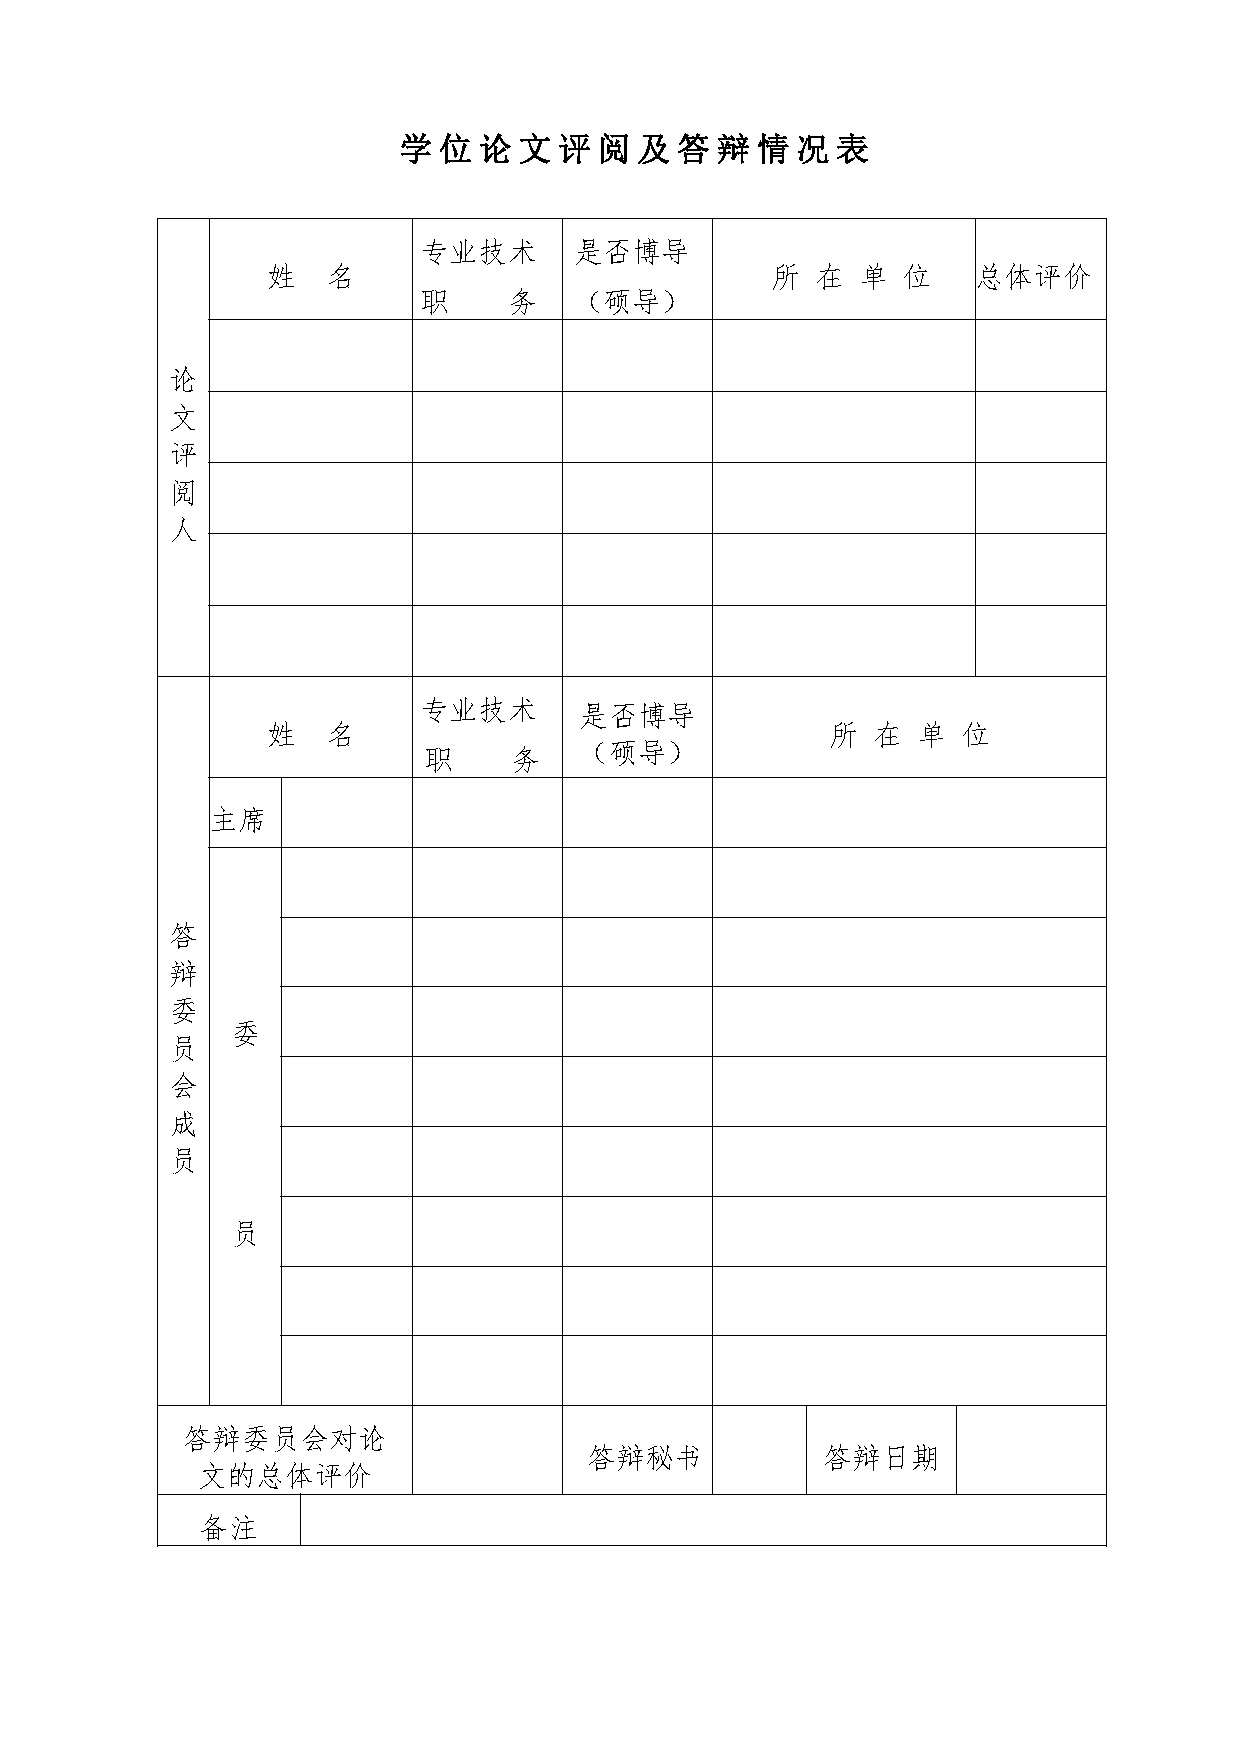
\includepdf[pages={1}]{fff.pdf}
	%\specialchap{外文论文}
\addcontentsline{toe}{chapter}{ENGLISH RESEARCH PAPER}

\end{document}

% vim:ts=4:sw=4
